\documentclass{beamer}

\usepackage{graphicx}
\usepackage{hyperref}
\usepackage[latin1]{inputenc}
\usepackage[T1]{fontenc}
\usepackage[english]{babel}
\usepackage{listings}
\usepackage{xcolor,mathrsfs,url}
\usepackage{amssymb}
\usepackage{amsmath}
\usepackage{ifthen}


% The command to define a subsection is '\subsec{}' and NOT '\subsection'.
% This code generates the bar. Don't edit.
\newcommand{\midbarnew}{}
\newcommand{\subsec}[1]
{
  \ifthenelse{\equal{#1}{}}
  {\renewcommand{\midbarnew}{} \subsection{}}
  {\renewcommand{\midbarnew}{ $\mid$ } \subsection{#1}}
}

% change the pictures here, if necessary. logobig and logosmall are the internal names
% for the pictures: do not modify them, just change "hulogo" and "logo". Pictures must be 
% supplied as JPEG, PNG or PDF
%########################################

\pgfdeclareimage[height=2cm]{logobig}{logo} % use hucase instead for the Humboldt-Case Logo
\pgfdeclareimage[height=1cm]{logosmall}{logo}

% use this number to modify the scaling of the headline on titlepage
\def\titlescale{1.0}


\title{Trade Policy: Part Two}
\author{Instructor: David Jinkins\thanks{I wish to acknowledge Battista Severgnini for providing last year's slides to me. His generosity saved me much time, and these slides are partially based on his. Any errors are of course my own.}}
\date{Date: Sept. 25, 2014}
%Start of the document
\begin{document}

\frame[plain]{% create the titleslide, layout controlled in metricsbeamer
	\titlepage
}

\frame{% how to print
\frametitle{Last time}
Chapter 8:
\begin{itemize}
\item Trade costs and Firm Behavior
\item Dumping
\item Multinationals
\end{itemize}
Chapter 9 : 
\begin{itemize}
\item Tariffs
\item Consumer \& Producer Surplus
\item Export Subsidies and other instruments
\end{itemize}
}

\frame{% how to print
\frametitle{Plan for Today}
\begin{itemize}
    \item Chapter 10 : Politics and Trade Policy
    \begin{itemize}
        \item Some additional arguments for Free Trade
        \item Arguments Against Free Trade
        \begin{itemize}
            \item National Welfare reasons 
            \item Income Distribution and Trade Policy
        \end{itemize}
        \item International Negotiations
        \begin{itemize}
            \item Some theory
            \item A short history of International Trade Agreements 
            \item Preferential Trade Arrangements
        \end{itemize}
    \end{itemize}
    \item Chapter 11 : Developing Countries and Trade Policy
    \begin{itemize}
        \item Rise and Fall of Import Substitution 
        \item Export Oriented Industrialization
    \end{itemize}
    \item Chapter 12: Trade Policy Controversy
    \begin{itemize}
        \item Arguments for an Activist Trade Policy
        \item Trade \& Labor
        \item Trade \& the Environment
    \end{itemize}
\end{itemize}
}

\begin{frame}{But first a Review}

    \begin{itemize}
        \item Begin review
    \end{itemize}

\end{frame}

\frame[plain]{\includegraphics[page=37,width=\textwidth]{trade_policy_one.pdf}}
\frame[plain]{\includegraphics[page=39,width=\textwidth]{trade_policy_one.pdf}}
\frame[plain]{\includegraphics[page=41,width=\textwidth]{trade_policy_one.pdf}}
\frame[plain]{\includegraphics[page=32,width=\textwidth]{trade_policy_one.pdf}}
\frame[plain]{\includegraphics[page=43,width=\textwidth]{trade_policy_one.pdf}}
\frame[plain]{\includegraphics[page=44,width=\textwidth]{trade_policy_one.pdf}}
\frame[plain]{\includegraphics[page=48,width=\textwidth]{trade_policy_one.pdf}}
\frame[plain]{\includegraphics[page=56,width=\textwidth]{trade_policy_one.pdf}}
\frame[plain]{\includegraphics[page=57,width=\textwidth]{trade_policy_one.pdf}}
\frame[plain]{\includegraphics[page=58,width=\textwidth]{trade_policy_one.pdf}}
\frame[plain]{\includegraphics[page=59,width=\textwidth]{trade_policy_one.pdf}}
\frame[plain]{\includegraphics[page=60,width=\textwidth]{trade_policy_one.pdf}}
\frame[plain]{\includegraphics[page=61,width=\textwidth]{trade_policy_one.pdf}}
\frame[plain]{\includegraphics[page=62,width=\textwidth]{trade_policy_one.pdf}}
\frame[plain]{\includegraphics[page=63,width=\textwidth]{trade_policy_one.pdf}}
\frame[plain]{\includegraphics[page=64,width=\textwidth]{trade_policy_one.pdf}}
\frame[plain]{\includegraphics[page=65,width=\textwidth]{trade_policy_one.pdf}}
\frame[plain]{\includegraphics[page=66,width=\textwidth]{trade_policy_one.pdf}}
\frame[plain]{\includegraphics[page=69,width=\textwidth]{trade_policy_one.pdf}}
\frame[plain]{\includegraphics[page=70,width=\textwidth]{trade_policy_one.pdf}}
\frame[plain]{\includegraphics[page=72,width=\textwidth]{trade_policy_one.pdf}}
\frame[plain]{\includegraphics[page=75,width=\textwidth]{trade_policy_one.pdf}}
\frame[plain]{\includegraphics[page=76,width=\textwidth]{trade_policy_one.pdf}}
\frame[plain]{\includegraphics[page=77,width=\textwidth]{trade_policy_one.pdf}}
\frame[plain]{\includegraphics[page=80,width=\textwidth]{trade_policy_one.pdf}}
\frame[plain]{\includegraphics[page=81,width=\textwidth]{trade_policy_one.pdf}}
\frame[plain]{\includegraphics[page=83,width=\textwidth]{trade_policy_one.pdf}}
\frame[plain]{\includegraphics[page=86,width=\textwidth]{trade_policy_one.pdf}}
\frame[plain]{\includegraphics[page=88,width=\textwidth]{trade_policy_one.pdf}}

\begin{frame}

    \begin{itemize}
        \item End review!
    \end{itemize}

\end{frame}

\begin{frame}{Chapter 10 : Politics and Trade Policy}

    \begin{itemize}
        \item Some additional arguments for Free Trade
        \item Arguments Against Free Trade
        \begin{itemize}
            \item National Welfare reasons 
            \item Income Distribution and Trade Policy
        \end{itemize}
        \item International Negotiations
        \begin{itemize}
            \item Some theory
            \item A short history of International Trade Agreements 
            \item Preferential Trade Arrangements
        \end{itemize}
    \end{itemize}

\end{frame}

\begin{frame}{Some more arguments for Free Trade}

\begin{itemize}
    \item Chap. 1-8: gains from trade
    \item What else?
    \begin{itemize}
        \item Stuff we sort of already talked about
        \item The rent seeking distortions
        \item Politics and corruption
    \end{itemize}
\end{itemize}

\end{frame}

\begin{frame}{Stuff we already mentioned}

    \begin{itemize}
        \item Efficiency losses for small countries making tariffs
        \item Economies of scale, trade barriers reduce market size 
        \item Innovation, hard to pick winners
        \item Gains from shifting production to more productive firms
    \end{itemize}

\end{frame}

\begin{frame}{Efficiency losses of tariff}

    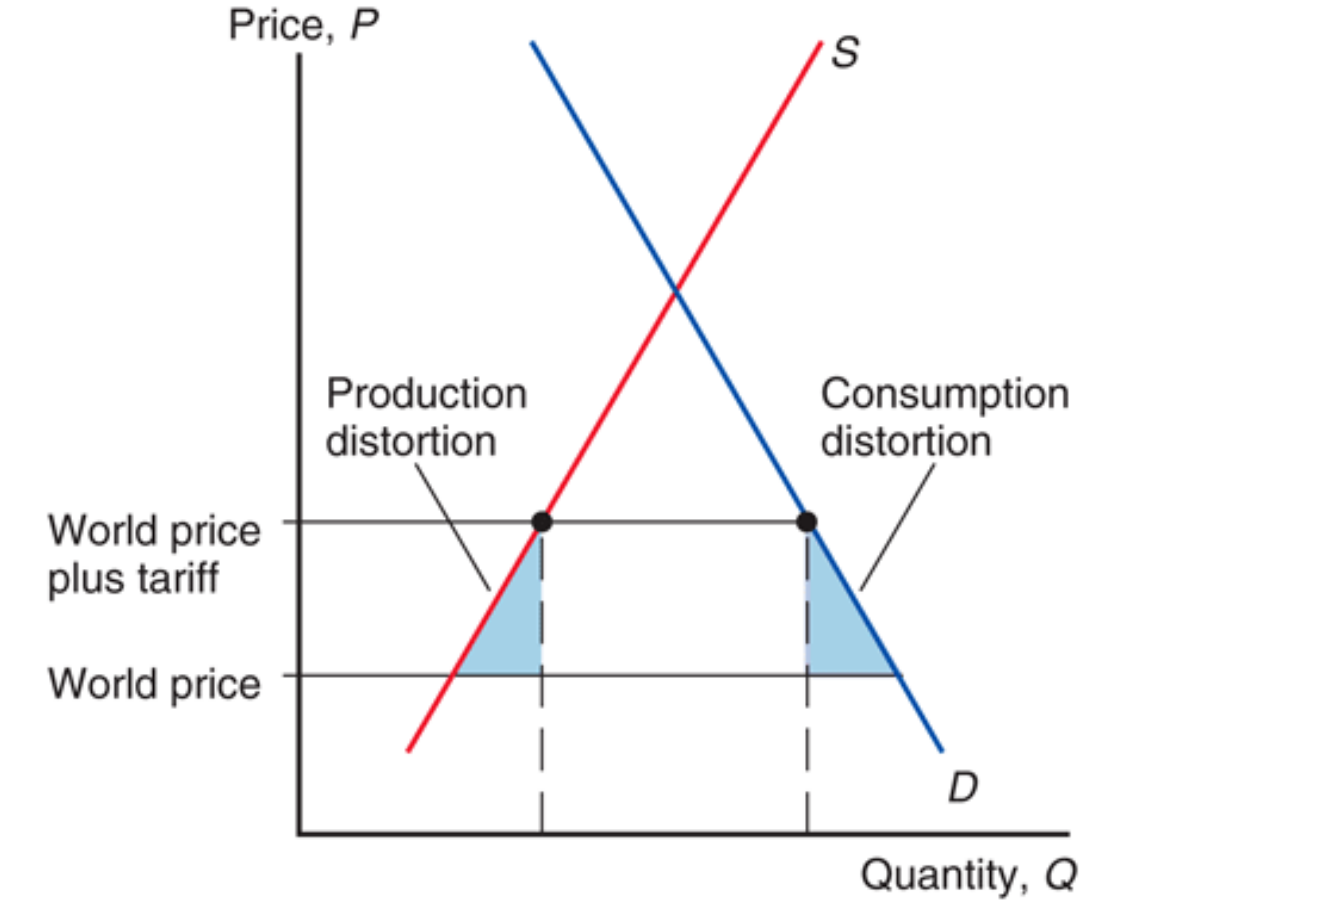
\includegraphics[scale=0.25]{tariff_distortion.png}

\end{frame}

\begin{frame}{Rent seeking distortions}

    \begin{itemize}
        \item Suppose we have import quotas
        \item How to allocate?
        \item Allocation system distorts production
        \begin{itemize}
            \item Example 1: India inport licenses based on capacity, build unneeded capacity
            \item Example 2: US Tuna import licenses first come first serve, warehouse in December, big rush on Jan. 1st
        \end{itemize}
        \item Side note: License Raj in India
    \end{itemize}

\end{frame}

\begin{frame}{Political Process and Corruption}

    \begin{itemize}
        \item Trade policy good in theory
        \item Politics is messy
        \begin{itemize}
            \item Even good intentioned policies likely to be captured by special interest groups
            \item Might cause even bigger distortions
            \item Here free trade is a second best 
        \end{itemize} 
        \item Similar argument to why one should follow unjust laws
    \end{itemize}

\end{frame}

\begin{frame}
    \begin{itemize}
% \frame{
% \frametitle{Political Models of Trade Policy}
% Models related to trade policy:
% \begin{enumerate}
% \item Median voter theorem
% \item Collective action
% \item A model of trade policy that combines aspects of the median voter theorem \& collective action
% \end{enumerate}
% }
% 
% \frame{
% \frametitle{Median Voter Theorem}
% Electoral competition can be modeled as:
% \begin{itemize}
% \item two parties
% \item $t_{m}$: equilibrium tariff 
% \item Both want majority $\Rightarrow$ both parties will offer the same tariff policy to court the median voter 
% \item \textbf{BUT} this model does not work well for trade policy (e.g. small groups/lobbies influence tariff, see Box at page 225)
% \end{itemize}
% }
% 
% \frame{
% \frametitle{Fig. 9-4: Political Competition}
% \begin{figure}
% 	\centering
% 		\includegraphics[width=0.80\textwidth]{91.pdf}
% 	\label{fig:11}
% \end{figure}
% }
% 
% \frame{
% \frametitle{Median Voter \& Tariffs}
% \begin{figure}
% 	\centering
% 		\includegraphics[width=0.80\textwidth]{mediumvoter.pdf}
% 	\label{fig:11}
% \end{figure}
% }
% 
% \frame{
% \frametitle{Collective Action (1)}
% Model introduced by Mancur Olson. Main assumptions:
% \begin{itemize}
% \item Political activity on behalf of a group is a \textit{public good}
% \item Policies with large aggregate/ total
% loss but small individual loss are
% difficult to change
% \item Collective action is required
% \end{itemize}
% }
% 
% 
% \frame{
% \frametitle{Collective Action (2)}
% \begin{figure}
% 	\centering
% 		\includegraphics[width=0.80\textwidth]{92.pdf}
% 	\label{fig:11}
% \end{figure}
% }
% 
% 
% \frame{
% \frametitle{A Model of Trade Policy}
% \begin{itemize}
% \item Politicians may win elections partly because they advocate popular policies (median voter theorem), but they also require funds to run campaigns (collective action)
% \item funds may especially come from groups who do not have a collective action problem and are willing to advocate a special interest policy
% \item models of trade restriction policy try to measure the trade off between the reduction in welfare of constituents as a whole and the increase in campaign contributions from special interests.
% \end{itemize}
% }
% 
% \frame{
% \frametitle{Which Industries are Protected?}
% \begin{itemize}
% \item Agriculture (Europe and Japan)
% \item Clothing (USA, about 14 \$ billion)
% \end{itemize}
% }
% 
% \Section{Chapter 9. International Negotiations}
% 
% \frame{
% \frametitle{International Negotiations}
% \begin{itemize}
% \item 1930: Smoot-Harley Act
% \item 1932: Bilateral negotiations
% \item 1947: Multilateral negotiations
% (GATT)
% \item 1995: WTO
% \end{itemize}
% }
% 
% \frame{
% \frametitle{Fig. 9-5: The U.S. Tariff Rate}
% \begin{figure}
% 	\centering
% 		\includegraphics[width=0.80\textwidth]{95.pdf}
% 	\label{fig:11}
% \end{figure}
% }
% 
% \frame{
% \frametitle{Multilateral Negotiations}
% \begin{itemize}
% \item Multilateral negotiations mobilize exporters to support free trade if they believe export markets will expand.
% \item Multilateral negotiations also help avoid a trade war between countries, where each country enacts trade restrictions.
% \item A trade war could result if each country has a political interest (due to political pressure) to protect domestic producers, regardless of what other countries do. 
% \end{itemize}
% }
% 
% \frame{
% \frametitle{Trade War }
% \begin{table}
% \begin{tabular}{c c||c c|c c||}
%  & & \multicolumn{4}{c||}{\textcolor{blue}{\textbf{European Union}}}\\\hline\hline
%  & &   \multicolumn{2}{c|}{Free Trade} & \multicolumn{2}{c||}{Protection}\\\hline
% \textcolor{red}{\textbf{US}}& Free trade &  &     &  &      \\\hline
% &  &       &  & &      \\\hline\hline
% \end{tabular}
% \end{table}
% }
% 
% \frame{
% \frametitle{Trade War }
% \begin{table}
% \begin{tabular}{c c||c c|c c||}
%  & & \multicolumn{4}{c||}{\textcolor{blue}{\textbf{European Union}}}\\\hline\hline
%  & &   \multicolumn{2}{c|}{Free Trade} & \multicolumn{2}{c||}{Protection}\\\hline
% \textcolor{red}{\textbf{US}}& Free trade &  & \textcolor{blue}{10B �}     &  &   \textcolor{blue}{20B �}   \\\hline
% &  &       &  & &       \\\hline\hline
% \end{tabular}
% \end{table}
% }
% 
% \frame{
% \frametitle{Trade War }
% \begin{table}
% \begin{tabular}{c c||c c|c c||}
%  & & \multicolumn{4}{c||}{\textcolor{blue}{\textbf{European Union}}}\\\hline\hline
%  & &   \multicolumn{2}{c|}{Free Trade} & \multicolumn{2}{c||}{Protection}\\\hline
% \textcolor{red}{\textbf{US}}& Free trade &  & \textcolor{blue}{10B �}     &  &   \textcolor{blue}{$\underline{20B �}$}   \\\hline
% &  &       &  & &        \\\hline\hline
% \end{tabular}
% \end{table}
% }
% 
% \frame{
% \frametitle{Trade War }
% \begin{table}
% \begin{tabular}{c c||c c|c c||}
%  & & \multicolumn{4}{c||}{\textcolor{blue}{\textbf{European Union}}}\\\hline\hline
%  & &   \multicolumn{2}{c|}{Free Trade} & \multicolumn{2}{c||}{Protection}\\\hline
% \textcolor{red}{\textbf{US}}& Free trade &  & \textcolor{blue}{10B �}     &  &   \textcolor{blue}{$\underline{20B �}$}   \\\hline
% \textcolor{red}{\textbf{US}}&Protection  &       & \textcolor{blue}{-10B �} & &  \textcolor{blue}{-5B �}      \\\hline\hline
% \end{tabular}
% \end{table}
% }
% 
% \frame{
% \frametitle{Trade War }
% \begin{table}
% \begin{tabular}{c c||c c|c c||}
%  & & \multicolumn{4}{c||}{\textcolor{blue}{\textbf{European Union}}}\\\hline\hline
%  & &   \multicolumn{2}{c|}{Free Trade} & \multicolumn{2}{c||}{Protection}\\\hline
% \textcolor{red}{\textbf{US}}& Free trade &  & \textcolor{blue}{10B �}     &  &   \textcolor{blue}{$\underline{20B �}$}   \\\hline
% \textcolor{red}{\textbf{US}}&Protection  &       & \textcolor{blue}{-10B �} & &  \textcolor{blue}{$\underline{-5B �}$}      \\\hline\hline
% \end{tabular}
% \end{table}
% }
% 
% 
% \frame{
% \frametitle{Trade War }
% \begin{table}
% \begin{tabular}{c c||c c|c c||}
%  & & \multicolumn{4}{c||}{\textcolor{blue}{\textbf{European Union}}}\\\hline\hline
%  & &   \multicolumn{2}{c|}{Free Trade} & \multicolumn{2}{c||}{\textcolor{blue}{Protection}}\\\hline
% \textcolor{red}{\textbf{US}}& Free trade &  & \textcolor{blue}{10B �}     &  &   \textcolor{blue}{$\underline{20B �}$}   \\\hline
% \textcolor{red}{\textbf{US}}&Protection  &       & \textcolor{blue}{-10B �} & &  \textcolor{blue}{$\underline{-5B �}$}      \\\hline\hline
% \end{tabular}
% \end{table}
% }
% 
% 
% 
% \frame{
% \frametitle{Trade War }
% \begin{table}
% \begin{tabular}{c c||c c|c c||}
%  & & \multicolumn{4}{c||}{\textcolor{blue}{\textbf{European Union}}}\\\hline\hline
%  & &   \multicolumn{2}{c|}{Free Trade} & \multicolumn{2}{c||}{\textcolor{blue}{Protection}}\\\hline
% \textcolor{red}{\textbf{US}}& Free trade & \textcolor{red}{10B �} & \textcolor{blue}{10B �}     &  &   \textcolor{blue}{$\underline{20B �}$}   \\\hline
% \textcolor{red}{\textbf{US}}&Protection  &  \textcolor{red}{20B �}     & \textcolor{blue}{-10B �} & &  \textcolor{blue}{$\underline{-5B �}$}      \\\hline\hline
% \end{tabular}
% \end{table}
% }
% 
% 
% \frame{
% \frametitle{Trade War }
% \begin{table}
% \begin{tabular}{c c||c c|c c||}
%  & & \multicolumn{4}{c||}{\textcolor{blue}{\textbf{European Union}}}\\\hline\hline
%  & &   \multicolumn{2}{c|}{Free Trade} & \multicolumn{2}{c||}{\textcolor{blue}{Protection}}\\\hline
% \textcolor{red}{\textbf{US}}& Free trade & \textcolor{red}{10B �} & \textcolor{blue}{10B �}     &  &   \textcolor{blue}{$\underline{20B �}$}   \\\hline
% \textcolor{red}{\textbf{US}}&Protection  &  $\textcolor{red}{\underline{20B �}}$     & \textcolor{blue}{-10B �} & &  \textcolor{blue}{$\underline{-5B �}$}      \\\hline\hline
% \end{tabular}
% \end{table}
% }
% 
% 
% \frame{
% \frametitle{Trade War }
% \begin{table}
% \begin{tabular}{c c||c c|c c||}
%  & & \multicolumn{4}{c||}{\textcolor{blue}{\textbf{European Union}}}\\\hline\hline
%  & &   \multicolumn{2}{c|}{Free Trade} & \multicolumn{2}{c||}{\textcolor{blue}{Protection}}\\\hline
% \textcolor{red}{\textbf{US}}& Free trade & \textcolor{red}{10B �} & \textcolor{blue}{10B �}     &  \textcolor{red}{$\underline{-10B �}$} &   \textcolor{blue}{$\underline{20B �}$}   \\\hline
% \textcolor{red}{\textbf{US}}&Protection  &  $\textcolor{red}{\underline{20B �}}$     & \textcolor{blue}{-10B �} & \textcolor{red}{$\underline{-5B �}$}&  \textcolor{blue}{$\underline{-5B �}$}      \\\hline\hline
% \end{tabular}
% \end{table}
% }
% 
% 
% \frame{
% \frametitle{Trade War }
% \begin{table}
% \begin{tabular}{c c||c c|c c||}
%  & & \multicolumn{4}{c||}{\textcolor{blue}{\textbf{European Union}}}\\\hline\hline
%  & &   \multicolumn{2}{c|}{Free Trade} & \multicolumn{2}{c||}{\textcolor{blue}{Protection}}\\\hline
% \textcolor{red}{\textbf{US}}& Free trade & \textcolor{red}{10B �} & \textcolor{blue}{10B �}     &  \textcolor{red}{$\underline{-10B �}$} &   \textcolor{blue}{$\underline{20B �}$}   \\\hline
% \textcolor{red}{\textbf{US}}& \textcolor{red}{Protection}  &  $\textcolor{red}{\underline{20B �}}$     & \textcolor{blue}{-10B �} & \textcolor{red}{$\underline{-5B �}$}&  \textcolor{blue}{$\underline{-5B �}$}      \\\hline\hline
% \end{tabular}
% \end{table}
% }
% 
% 
% \frame{
% \frametitle{"Ulysses and the Sirens" (1)}
% \textit{But if you wish to listen,
% let the men tie you in the lugger,, hand
% and foot, back to the mast, lashed to the mast,
% so you may hear those harpies' thrilling voices...}[Homer, Odyssey]
% \begin{figure}
% 	\centering
% 		\includegraphics[width=0.75\textwidth]{uly.pdf}
% 	\label{fig:11}
% \end{figure}
% }
% 
% 
% \frame{
% \frametitle{"Ulysses and the Sirens" (2)}
% If countries can establish a binding agreement to maintain free trade, both can avoid the temptation of protection and both can be made better off.
% $\Rightarrow$ World Trade Organization (WTO)
% \begin{enumerate}
% \item Reduction of tariff rates 
% \item Binding
% \item Prevention of non-tariff barriers
% \end{enumerate}
% }
% 
% \frame{
% \frametitle{Preferential Trade Agreement (1)}
% \begin{enumerate}
% \item \textbf{free trade area:} an agreement that allows free trade among members, but each member can have its own trade policy towards non-member countries (e.g., NAFTA)
% \item \textbf{custom unions:} an agreement that allows free trade among members and requires a common external trade policy towards non-member countries. (e.g., European Union)
% \end{enumerate}
% }
% 
% 
% 
% \frame{
% \frametitle{Preferential Trade Agreement (2)}
% \begin{table}
% \begin{tabular}{||l|c|c|c|c||}\hline \hline
%  & \textbf{UK} & \textbf{F} & \textbf{US} & \textbf{UK import from}\\ \hline
% $p$ & 8 & 6 & 4 & US \\ \hline
% \multicolumn{5}{||c||}{$1^{st}$ case}\\ \hline
% $p+t$ & 8 & 11 & 9 & -\\
% CU with F & 8 & 6 & 9 & F (trade creation)\\ \hline
% \multicolumn{5}{||c||}{$2^{nd}$ case}\\ \hline
% $p+t^{2}$ & 8 & 9 & 7 & US\\
% CU with F & 8 & 6 & 7 & F (trade diversion)\\ \hline
% \end{tabular}
% \end{table}
% }
% 
% 
% 
% \Section{Chapter 10. Import Substituting Industrialization}
% \frame{% how to print
% \frametitle{}
% \begin{center}
% \textcolor{blue}{\Huge{\textbf{Chapter 10: Trade Policy in Developing Countries
% }}}
% \end{center}
% }
% 
% \frame{% how to print
% \frametitle{Developing Countries}
% Developing countries:
% \begin{itemize}
% \item many low and middle income countries
% \item not precise definition
% \end{itemize}
% }
% 
% \frame{% how to print
% \frametitle{Import Substituting Industrialization}
% Developing countries:
% \begin{itemize}
% \item trade policy adopted by many developing countries before the 1980s (e.g., in Latin America 1950-60)
% \item encourage domestic industries (\textit{infant industries}) by limiting competing imports
% \item common belief: poor countries would be exploited by rich countries through international financial markets and trade.
% \end{itemize}
% but
% \begin{enumerate}
% \item comparative advantages
% \item firms could be uncompetitive
% \item market failures
% \end{enumerate}
% }
% 
% 
% \frame{% how to print
% \frametitle{Infant Industries and Market Failures}
% Two arguments for how market failures prevent infant industries from becoming competitive:
% \begin{enumerate}
% \item Imperfect financial asset markets
% \item The problem of appropriability 
% \end{enumerate}
% }
% 
% \Section{Chapter 10. Free Trade}
% 
% \frame{% how to print
% \frametitle{Trade Liberalization}
% There is some evidence that low and middle income countries which had relatively free trade had higher average economic growth than those that followed import substituting industrialization (after mid-1980s).
% }
% 
% 
% \frame{
% \frametitle{Table 10-3: Effective Rates of Protection for Manufacturing in India and Brazil}
% \begin{figure}
% 	\centering
% 		\includegraphics[width=0.80\textwidth]{table1.pdf}
% 	\label{fig:11}
% \end{figure}
% }
% 
% 
% \frame{
% \frametitle{Fig. 10-1: The Growth of Developing-Country Trade}
% \begin{figure}
% 	\centering
% 		\includegraphics[width=0.80\textwidth]{graf1.pdf}
% 	\label{fig:11}
% \end{figure}
% }
% 
% \frame{
% \frametitle{Has Trade Liberalization Promoted Development?}
% \begin{itemize}
% \item Mixed evidence (free trade bad for Latin America).
% \item but difficult to disentangle trade from financial crises
% \item more income inequality (prediction from Hechscher-Ohlin model)
% \end{itemize}
% }
% 
% \Section{Chapter 10. Export Oriented Industrialization}
% 
% \frame{
% \frametitle{Export Oriented Industrialization}
% \begin{itemize}
% \item "high performance Asian economies" adopted trade policies that promoted exports in targeted industries
% \item Although evidence suggests that these economies did have less restricted trade than other low and middle income countries, some trade restrictions were sometimes still in effect. (causality or correlation ?)
% \end{itemize}
% }
% 
% 
% \frame{
% \frametitle{Table 10-4: Average Rates of Protection, 1985 (percent)}
% \begin{figure}
% 	\centering
% 		\includegraphics[width=0.80\textwidth]{tab2.pdf}
% 	\label{fig:11}
% \end{figure}
% }
% 
% 
% \Section{Chapter 11. Controversies in Trade Policy}
% \frame{% how to print
% \frametitle{}
% \begin{center}
% \textcolor{blue}{\Huge{\textbf{Chapter 11: Controversies in Trade Policy
% }}}
% \end{center}
% }
% 
% \Section{Chapter 11. Arguments for an Activist Trade Policy}
% 
% \frame{
% \frametitle{Arguments for an Activist Trade Policy}
% \begin{enumerate}
% \item market failure
% \item infant industry
% \item technologies \& externalities
% \item imperfect competition
% \end{enumerate}
% }
% 
% \frame{
% \frametitle{Technology \& Externalities}
% Governments may want to actively encourage investment in technology when externalities in new technologies create a high marginal social benefit.
% Problem: Governments ability to target the right
% thing
% \begin{enumerate}
% \item Which industries do R\&D (high-tech industries (!?))
% \item Screening.
% \item Jones and Williams (1998): \textit{[The results]
% imply a conservative estimate of optimal/actual of
% about 4�}
% \end{enumerate}
% }
% 
% \frame{
% \frametitle{Imperfect Competition and Strategic Trade Policy}
% \begin{itemize}
% \item Imperfectly competitive industries are typically dominated by a few firms that generate monopoly profits or excess profits (or excess returns).
% \item In an imperfectly competitive industry, government subsidies can shift excess profits from a foreign firm to a domestic firm.
% \end{itemize}
% }
% 
% 
% 
% \frame{
% \frametitle{Profit Steeling (1)}
% Suppose Boeing enters the market first and it decides to produce
% \begin{table}
% \begin{tabular}{c c||c c|c c||}
%  & & \multicolumn{4}{c||}{\textcolor{blue}{\textbf{Airbus}}}\\\hline\hline
%  & &   \multicolumn{2}{c|}{Produce} & \multicolumn{2}{c||}{\textcolor{blue}{Not Produce}}\\\hline
% \textcolor{red}{\textbf{Boeing}}& \textcolor{red}{Produce} & \textcolor{red}{-5} & \textcolor{blue}{-5}     &  \textcolor{red}{$\underline{100}$} &   \textcolor{blue}{$\underline{0}$}   \\\hline
% \textcolor{red}{\textbf{Boeing}}& Not Produce  &  $\textcolor{red}{{0}}$     & \textcolor{blue}{100} & \textcolor{red}{0}&  \textcolor{blue}{0}      \\\hline\hline
% \end{tabular}
% \end{table}
% }
% 
% \frame{
% \frametitle{Profit Steeling (2)}
% \begin{itemize}
% \item EU subsidize production by 25
% \item Airbus will also produce independent of Boeing's decision
% \item Boeing knows that and decides not to produce
% \item $125 > 25 \Rightarrow$ social benefit
% \end{itemize}
% \begin{table}
% \begin{tabular}{c c||c c|c c||}
%  & & \multicolumn{4}{c||}{\textcolor{blue}{\textbf{Airbus}}}\\\hline\hline
%  & &   \multicolumn{2}{c|}{\textcolor{blue}{Produce}} & \multicolumn{2}{c||}{Not Produce}\\\hline
% \textcolor{red}{\textbf{Boeing}}& Produce & \textcolor{red}{-5} & \textcolor{blue}{20}     &  \textcolor{red}{100} &   \textcolor{blue}{0}   \\\hline
% \textcolor{red}{\textbf{Boeing}}& \textcolor{red}{Not Produce}  &  \textcolor{red}{$\underline{0}$}     & \textcolor{blue}{$\underline{125}$} & \textcolor{red}{0}&  \textcolor{blue}{0}      \\\hline\hline
% \end{tabular}
% \end{table}
% }
% 
% \frame{
% \frametitle{Profit Steeling (3)}
% \begin{itemize}
% \item "beggar-thy-neighbor"
% \end{itemize}
% \begin{table}
% \begin{tabular}{c c||c c|c c||}
%  & & \multicolumn{4}{c||}{\textcolor{blue}{\textbf{Airbus}}}\\\hline\hline
%  & &   \multicolumn{2}{c|}{\textcolor{blue}{Produce}} & \multicolumn{2}{c||}{Not Produce}\\\hline
% \textcolor{red}{\textbf{Boeing}}& \textcolor{red}{Produce} & \textcolor{red}{$\underline{5}$} & \textcolor{blue}{$\underline{5}$}     &  \textcolor{red}{125} &   \textcolor{blue}{0}   \\\hline
% \textcolor{red}{\textbf{Boeing}}& Not Produce  &  \textcolor{red}{0}     & \textcolor{blue}{125} & \textcolor{red}{0}&  \textcolor{blue}{0}      \\\hline\hline
% \end{tabular}
% \end{table}
% }
% 
% \Section{Chapter 11. Trade \& Labor}
% 
% \frame{
% \frametitle{Trade \& Labor}
% \begin{itemize}
% \item Compared to rich country standards, workers who produce these goods are paid low wages and may work under poor conditions.
% \item Some have opposed free trade because of this fact.
% \item Predictions: Ricardo vs. Heckscher-Ohlin model 
% \end{itemize}
% }
% 
% \Section{Chapter 11. Trade \& Environment}
% \frame{
% \frametitle{Trade \& Environment (1)}
% \begin{itemize}
% \item Compared to rich country standards, environmental standards in low and middle income countries are lax.
% \item Some have opposed free trade because of this fact.
% \end{itemize}
% }
% 
% 
% \frame{
% \frametitle{Trade \& Environment (2)}
% \begin{itemize}
% \item As poor countries grow richer, possibly partly due to trade, they produce more and can consume more, leading to more environmental degradation. 
% \item But as countries grow richer, they want to pay for more stringent environment protection.
% \item \textbf{environmental Kuznets curve}
% \end{itemize}
% }
% 
% \frame{
% \frametitle{Fig. 11-1: The Environmental Kuznets Curve}
% \begin{figure}
% 	\centering
% 		\includegraphics[width=0.80\textwidth]{kuz.pdf}
% 	\label{fig:11}
% \end{figure}
% }
% 
% 
% \frame{
% \frametitle{Figure: VER and Pollution (Source: Feenstra and Taylor (2010)}
% \begin{figure}
% 	\centering
% 		\includegraphics[width=0.80\textwidth]{japancar.pdf}
% 	\label{fig:11}
% \end{figure}
% }
% 
% \frame{
% \frametitle{Figure: Trade in Bufalo (Source: Scott Taylor (2007)}
% \begin{figure}
% 	\centering
% 		\includegraphics[width=0.80\textwidth]{bufalo.pdf}
% 	\label{fig:11}
% \end{figure}
% }
% \frame{
% \frametitle{Suggested Articles}
% \begin{footnotesize}
% \begin{thebibliography}{aaaaaaaaaaaaaaaaa}
% \beamertemplatebookbibitems
% \bibitem[Feenstra, 2003]{haerdle2003}
% Elster, J.
% \newblock {\em Ulysses and the Sirens: Studies in Rationality and Irrationality}
% \newblock Cambridge Paperback Library, 1987
% \beamertemplatearticlebibitems
% \bibitem[Jones]{jones1982}
% Jones, C.I., Williams, J.C.
% \newblock Measuring the social return to R\&D,
% \newblock The Quarterly Journal of Economics, vol. 113(4), pages 1119-1135, November 1998
% \beamertemplatebookbibitems
% \bibitem{rourke}
% Ostrom, Elinor 
% \newblock {\em Governing the Commons: The Evolution of Institutions for Collective Action}
% \newblock Cambridge University Press, 1990
% \end{thebibliography}
% \end{footnotesize}
% }

\end{document}
